\documentclass{thesis}
\usepackage{graphicx}
%\usepackage[dvipdfmx]{graphicx}
\usepackage[dvipdfmx]{color}
\usepackage{float}
\usepackage{listings}
\usepackage{jvlisting} %日本語のコメントアウトをする場合jvlisting(もしくはjlisting)が必要
\usepackage{amsmath}
\usepackage{mathtools}
\usepackage{stmaryrd} % \llparenthesis & rrparenthesis
\usepackage[dvipsnames]{xcolor}
\allowdisplaybreaks
%ここからソースコードの表示に関する設定
\lstset{
  basicstyle={\ttfamily},
  identifierstyle={\small},
  commentstyle={\smallitshape},
  keywordstyle={\small\bfseries},
  ndkeywordstyle={\small},
  stringstyle={\small\ttfamily},
  frame={tb},
  breaklines=true,
  columns=[l]{fullflexible},
  numbers=left,
  xrightmargin=0zw,
  xleftmargin=3zw,
  numberstyle={\scriptsize},
  stepnumber=1,
  numbersep=1zw,
  lineskip=-0.5ex
}
%\usepackage{xcolor}
%%%%%%%%%%%%%%%%%%%%%%%%%%%%%%%%%%%%%%%%%%%%%%%%%%
%%% 基本設定

%目次を表示するには2回コンパイルが必要!!

\論文名{2024年度 卒業/修士論文(中間発表)}
\所属{岐阜大学大学院工学研究科 応用情報学専攻 草刈研究室}
\学生番号{1224525023}
\氏名{恩田晴登}
\指導教員{草刈圭一朗}
\題目{mypyによる静的型検査を活用したPythonベースのコレオグラフィック言語の実装}
\日付{2023年12月19日}

%%%%%%%%%%%%%%%%%%%%%%%%%%%%%%%%%%%%%%%%%%%%%%%%%%
%%% ユーザ定義

% …… ご自由に定義してください ……
\renewcommand{\lstlistingname}{プログラム}
\newcommand{\projection}[2]{{\color{cyan}\llparenthesis}#1{\color{cyan}\rrparenthesis^#2}}
\newcommand{\gray}[1]{\textbf{\textsf{\color{Gray}#1}}}
\newcommand{\cyan}[1]{\color{cyan}#1}
\newcommand{\gr}[1]{\color{ForestGreen}#1}
\newcommand{\nl}[1]{{\color{red}{\llbracket}}#1{\color{red}{\rrbracket}}} % Normalizer symbol
\newcommand{\mg}{~{\color{red}{\sqcup}}~} % Merging symbol
%%%%%%%%%%%%%%%%%%%%%%%%%%%%%%%%%%%%%%%%%%%%%%%%%%
%%% 本文
\begin{document}

\maketitle %表紙
\frontmatter\tableofcontents\mainmatter %目次

%%%%%%%%%%%%%%%%%%%%%%%%%%%%%%%%%%%%%%%%%%%%%%%%%%%%%%%%%%%%
%%% はじめに
\chapter{はじめに}
%論証したいStatementを記述
%\begin{itemize}
%  \item Pythonは機械学習やIoTの業界で盛んに使用されているプログラミング言語の一つである
%  \item Pythonはマルチスレッドによる並行動作はGil(global interpreter lock)があるため行えない
%  \item しかし、近いうちにPythonからGilが排除される予定があり、Pythonでマルチスレッドプログラムを書く人が増えるだろう
%  \item ただ、一般的にマルチスレッドプログラムをデッドロックなどのエラーを出さずに書くのは困難
%  \item 単一のプログラムとしてマルチパーティなプロトコルを記述し、並行性起因のエラーが出ないようなコレオグラフィック言語があれば、不安/問題が解消される
%  \item Pythonベースのコレオグラフィック言語を実装する。
%  \item この際にJavaを拡張したコレオグラフィック言語であるChoralを参考にする。
%\end{itemize}
Pythonは機械学習やIoTの業界で盛んに使用されているプログラミング言語の一つである。Pythonは現在、グローバル・インタプリタ・ロック(GIL)が存在する。
これは、一度に1つのスレッドだけがPythonバイトコードを実行することを保証するためにCPythonインタプリタによって使用されるメカニズムである。
これにより、オブジェクトモデルが同時アクセスに対して暗黙的に安全になり、インタプリタのマルチスレッド化が容易になるが、弊害としてマルチプロセッサマシンによってもたらされる並列処理の多くが犠牲になる。

しかし、近い将来PythonはGILの除去可能性があることを発表した。その影響によりPythonユーザーがマルチスレッド環境でのプログラミングをすることが増えるであろう。
ただ、一般的に並列処理を用いたプログラムはデッドロックなどのエラーを出さずに記述することは困難であるため、バグが大量に出てくる恐れがある。
よって、単一のプログラムとしてマルチパーティなプロトコルを記述し、デッドロック等の並行性起因エラーが起こらないことが保証されているコレオグラフィック言語があれば、多くのPythonプログラマーの不安や負担が解消される。

本研究では、先行研究であるJavaを拡張したコレオグラフィックプログラミング言語Choralの理論を参考に、Pythonベースのコレオグラフィックプログラミング言語であるPyChoralの実装を行い、マルチスレッドプログラムをPythonで書くプログラマにとっての有用性を示す。
%%%%%%%%%%%%%%%%%%%%%%%%%%%%%%%%%%%%%%%%%%%%%%%%%%
\chapter{コレオグラフィックプログラミング}
本研究で実装するPyChoralはコレオグラフィックプログラミング言語の一つである。この章では本研究に関する前提知識と先行研究について述べる。
%%%%%%%%%%%%%%%%%%%%%%%%%%%%%%%%
\section{コレオグラフィーとエンドポイント射影}
コレオグラフィーとは、並行に動作する複数の参加者の連携手順をまとめたプログラムパラダイムである。
これにより、デッドロック等の並行性起因のエラーが起こる恐れを排除できる。
コレオグラフィーに従った各エンドポイント(通信の参加者)の型情報はエンドポイント射影という動作により、自動的に抽出される。
\begin{figure}[H]
  \centering
  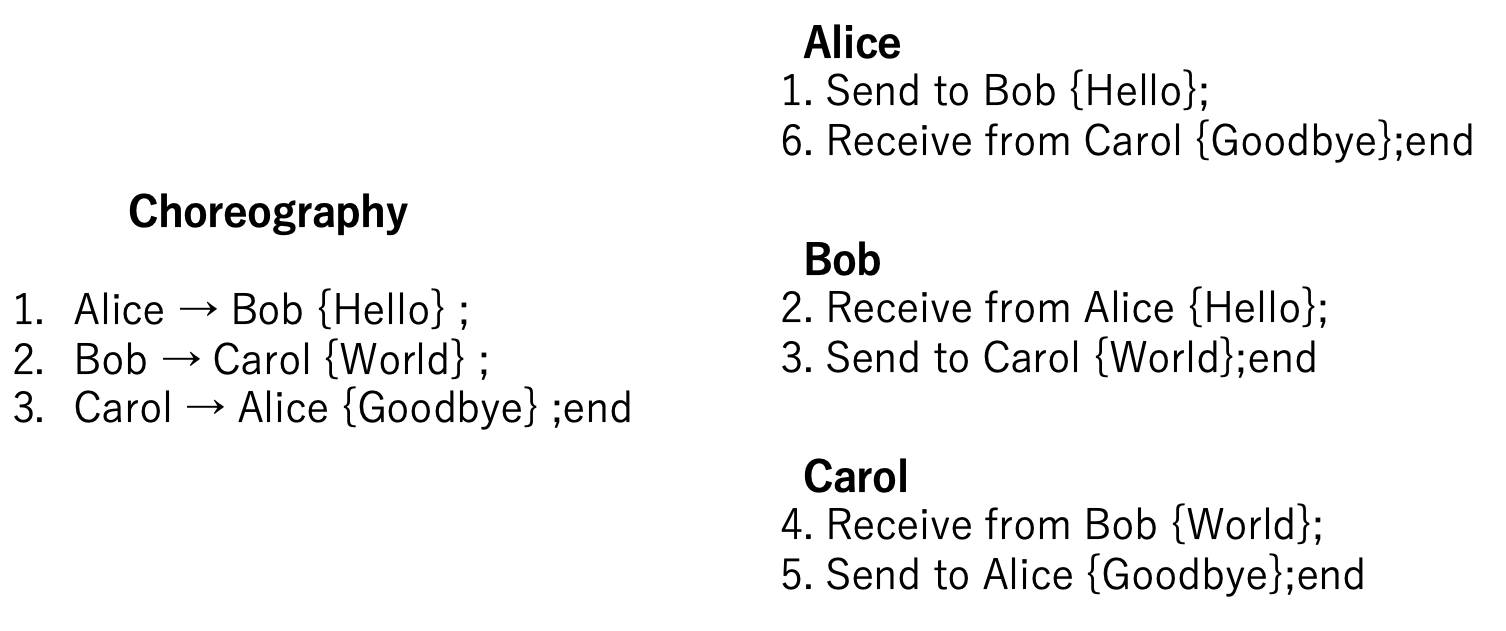
\includegraphics[scale=0.5]{image/choreography.png}
  \caption{コレオグラフィーとエンドポイント(Alice,Bob,Carolの会話)}
\end{figure}
ただし、通常のコレオグラフィーはコンパイル時にエンドポイントの型情報を導出するだけであり、そこからプログラマーが手動で
導出した型情報を元に各エンドポイントのプログラムを記述しなければならないため、バグが起きた際の処理などがプログラマーにとって負担になってしまうという難点がある。

エンドポイント射影とは、コレオグラフィーから各参加者の型情報を導出する操作である。
コレオグラフィックプログラミング言語にはコンパイラが付属しており、コンパイラはエンドポイント射影理論によって同時分散システム用の実行可能コードに変換する。

\begin{figure}[H]
  \centering
  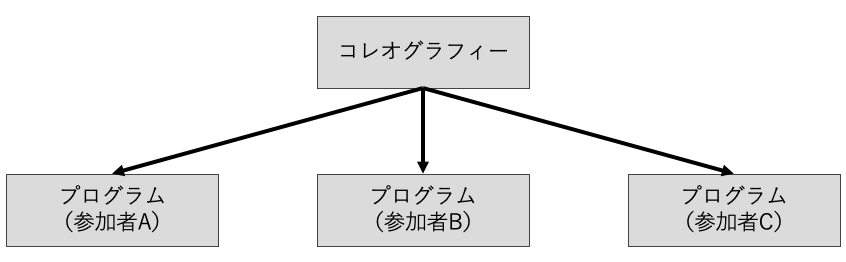
\includegraphics[scale=0.8]{image/epp.png}
  \caption{エンドポイント射影(参加者3人)}
\end{figure}
%%%%%%%%%%%%%%%%%%%%%%%%%%%%%
\section{Choral}
ChoralはJavaをベースとしたコレオグラフィックプログラミング言語である。前節で述べたように、
マルチスレッド環境で動作するプログラムでは、データ競合が発生しないようにするのがプログラマの責任であり大きな負担となっていたが、
Choralは、分散システムに従わせたいプロトコル全体を単一のプログラムとして作成できるため、これらの負担が軽減される。
Choralのオブジェクトには$t@(R_1,\cdots,R_n)$という形式の型があり、Javaの基本的なオブジェクトインターフェイス$T$に
各参加者の情報となるパラメータ$R_1,\cdots,R_n$が存在する。これにより、Choralプログラムをコンパイルする際に各参加者のプログラムが、
コレオグラフィーに従った形で自動的に生成することができる。

以下はChoralのプログラム例とChoralコンパイラによって自動導出されるJavaプログラムの一例である。
\begin{lstlisting}[caption=Choralプログラムの例(分散認証),label=choral]
enum AuthBranch { Ok,KO }

public class DistAuth@(Client,Service,IP){
  private TLSChannel@(Client,IP)<object> ch_Client_IP; #aaあa
  private TLSChannel@(Service,IP)<object> ch_Service_IP;
  ...
  public AuthResult@(Client,Service) authenticate(Credentials@Client credentials) {
    String@Client salt = ch_Client_IP.<String>com(ClientRegistry@IP.getSalt(ch_Client_IP.<String>com(credentials.username)));
    Boolean@IP valid = ClientRegistry@IP.check(ch_Client_IP.<String>com(calcHash(salt, credentials.password)));
    if (valid) {
      ch_Client_IP.<AuthBranch>select(AuthBranch@IP.OK);
      ch_Service_IP.<AuthBranch>select(AuthBranch@IP.OK);
      AuthToken@IP t = AuthToken@IP.create();
      return new AuthResult@(Client,Service)(
      ch_Client_IP.<AuthToken>com(t), ch_Service_IP.<AuthToken>com(t)
      );
    } else {
      ch_Client_IP.<AuthBranch>select(AuthBranch@IP.KO);
      ch_Service_IP.<AuthBranch>select(AuthBranch@IP.KO);
      return new AuthResult@(Client,Service)();
    }
  }
}
\end{lstlisting}
\ref{choral}はClient,Service,IPの3つの役割からなる分散認証システムを簡約したものである。
Choralプログラムはクラス名や変数、型などに$@$でロール名の情報を加えている。
また、ChoralにはJavaにはないcomメソッドとselectionメソッドなるものがある。

\begin{lstlisting}[caption=データ転送のための基本的な有向チャンネル,label=com]
interface DiDataChannel@(A,B)<T@C> {
  <S@D extends T@D> S@B com(S@A m);
} 
\end{lstlisting}
\ref{com}はcomメソッドの最も簡易的に使用しているインターフェースの例である。DiDataChannelは、
AとBで抽象化された2つのロール間の有向チャンネルで、型パラメータTで抽象化された型のデータをAからBに転送するための
インターフェースである。データ転送はcomを呼び出すことによって実行される。comは、Aに位置するTのサブタイプの任意の値S@Aを取り、S@Bを返す。
例えば\ref{choral}の8行目の外側のcomはClientからIPへString型のメッセージ(credentional@IP.getsalt(...))を転送することを意味する。

\begin{lstlisting}[caption=selectionメソッドの定義,label=select]
interface DiSelectChannel@(A,B) {
  @SelectionMethod
  <T@C extends Enum@C<T>> T@B select(T@A m);
} 
\end{lstlisting}
selectionメソッドはロール間で列挙型のインスタンスを送信する際に使用する。
例えば、\ref{choral}の11行目、18行目ではClientからIPへ列挙型の値OK,KOを転送することを意味する。
selectionメソッドは選択を意味し、プロジェクション後はswitch文としてJavaプログラムに現れる(\ref{java})。
\begin{lstlisting}[caption=生成されたClientのJavaプログラム(分散認証),label=java]
public class DistAuth_Client {
  private TLSChannel_A<Object> ch_Client_IP;

  public DistAuth_Client(TLSChannel_A <Object> ch_Client_IP) {
    this.ch_Client_IP = ch_Client_IP;
  }

  private String calcHash( String salt, String pwd ) { /*...*/ }

  public AuthResult_A authenticate(Credentials credentials) {
    String salt = ch_Client_IP.<String>com(ch_Client_IP.<String>com(credentials.username));
    ch_Client_IP.<String>com(calcHash(salt, credentials.password));
    switch (ch_Client_IP.<AuthBranch>select(Unit.id)) {
      case OK -> { return new AuthResult_A( ch_Client_IP.<AuthToken>com(Unit.id), Unit.id); }
      case KO -> { return new AuthResult_A(); }
      default -> { throw new RuntimeException( /*...*/ ); }
    }
  }
}
\end{lstlisting}
Client,Service,IPのうち、Clientにプロジェクションすると\ref{java}が生成される。Javaプログラムには@が存在せず、
ChoralプログラムでClientが関係する式や文のみ射影後に残る。\ref{choral}の10〜21行目のif文は\ref{java}の14〜17行目
のswitch文に変換されており、caseは列挙型の値で場合分けされて、それぞれif節とelse節のreturn文をもつ。

このようにChoralプログラムからコンパイラーを通して各エンドポイントのJavaプログラムが自動導出される。それぞれのJavaプログラムは
コレオグラフィーに従っているため、相互関係によるバグがないことが保証されている。これは、マルチパーティなプロトコルを記述するJavaプログラマーにとっては大きなメリットである。

%%%%%%%%%%%%%%%%%%%%%%%%%%%%%%%%%%%%%%%%%%%%%%%%%%
\chapter{mypy}
%\begin{itemize}
%  \item mypyはPythonの静的型検査器であり、既存のPythonコードに型アノテーションを追加することで、型が誤っていると警告を出すようになる。
%  \item Pythonは動的型付け言語であるため実行時にのみエラーが表示されるが、mypyにより実行しなくてもコンパイル時にバグが検出できる。
%  \item mypyの仕組み(プログラム→抽象構文木→型検査→エラー)← 図でやる
%\end{itemize}
Pythonは動的型付け言語で実行時にのみエラーが表示されるのでコンパイル時に型に対するエラーは表示されない。
mypyはPythonの静的型検査器であり、既存のPythonコードに型アノテーションを追加することで、型が誤っていると警告を出すようになる。
これによりコンパイル時にバグの検出が可能になり、安全なコーディングが可能となる。
\begin{lstlisting}[caption=型注釈のないPythonコード]
def greeting(name):
  return 'Hello ' + name

greeting(123)
greeting(b"Alice")
\end{lstlisting}
\begin{lstlisting}[caption=型注釈のあるPythonコード]
def greeting(name: str) -> str:
  return 'Hello ' + name

greeting("World!")  # No error
greeting(3)         # Argument 1 to "greeting" has incompatible type "int"; expected "str"
greeting(b'Alice')  
# Argument 1 to "greeting" has incompatible type "bytes"; expected "str"
\end{lstlisting}
本研究ではmypyを別のPythonアプリケーションに統合するために、Pythonプログラムにmypy.apiをインポートして型検査を行う。
以下は通常のmypyを使用した際の型検査のプロセスである。
\begin{figure}[H]
  \centering
  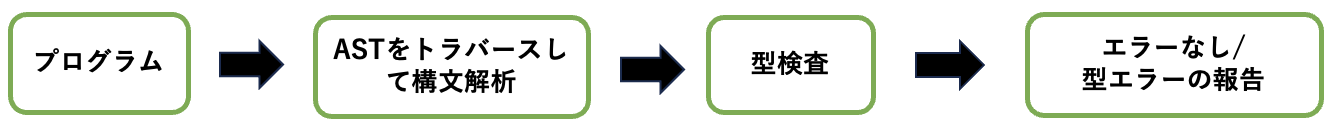
\includegraphics[scale=0.6]{image/mypyprocess.png}
  \caption{mypyプロセス}
\end{figure}
%%%%%%%%%%%%%%%%%%%%%%%%%%%%%%%%%%%%%%%%%%%%%%%%%%
\chapter{PyChoral}
\section{PyChoralの概要}
%\begin{itemize}
%  \item PyChoralはPythonベースのコレオグラフィックプログラミング言語
%  \item Choralは独自のコンパイラを作成し、Javaプログラムに型情報として参加者の情報を$@$で記述していたが、
%  PyChoralではPythonのパーサーをそのまま用いるため、$@$で参加者の情報を加えられない。→ 使えるようにする
%  \item mypyを活用したPyChoralでのプロセス(mypyをどう変えて使っているか)
%\end{itemize}
PyChoralはPythonベースのコレオグラフィックプログラミング言語である。PyChoralでマルチパーティなプログラムを記述し、
コンパイルすることで型エラーがない場合は、各参加者のPythonプログラムコードがコレオグラフィーに従った形で自動導出することができる。

PyChoralではmypyを活用した型検査のプロセスを改造し、型検査を行なった後に各エンドポイントのASTを再構築し、各エンドポイントのPythonプログラムを生成する。
\begin{figure}[H]
  \centering
  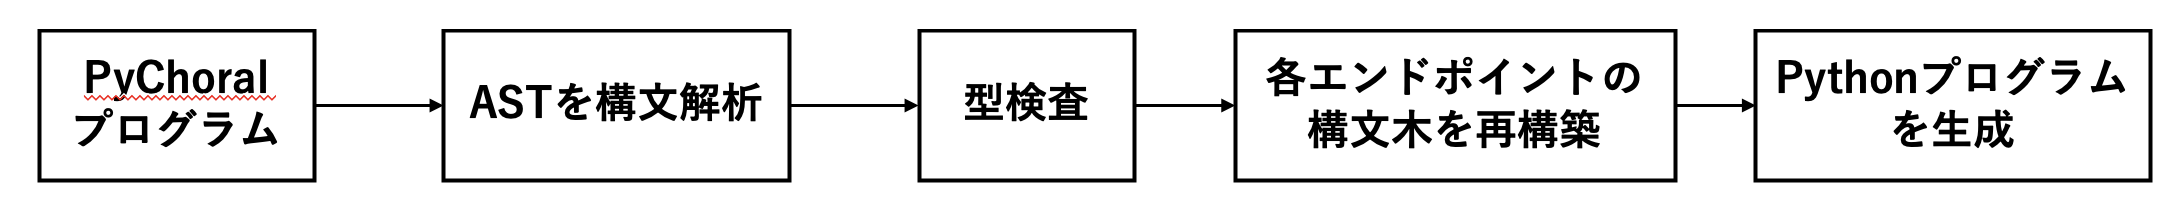
\includegraphics[scale=0.5]{image/pychoralprocess.png}
  \caption{PyChoralプロセス}
\end{figure}
PyChoralはPythonベースの言語のため、JavaベースのChoralを模倣するには静的型付け言語として扱え、コンパイル時にエラーの有無を判別したいためMypyを活用する。
ただし、Mypyで型注釈をつけらればChoralと同じように動くかというと、そうではない。

まず、ChoralはJavaのパーサーを改良し、独自のコンパイラーを使用してChoralプログラムからJavaプログラムを自動導出しているが、
本研究では既存のPythonパーサーをそのまま活用できるようにした。

Choralを真似するだけではだめ! Choralとの違い、苦労した点などを書く。
\begin{itemize}
  \item mypytestでのプロジェクションの仕方
  \item @をどうしたか
  \item Atクラス追加
\end{itemize}

\section{PyChoralによるプログラム例}
ChoralのAuthDistを参照した。(まだ実際はできていない)

プログラムの説明をここに書く。
\begin{lstlisting}[caption=PyChoralプログラムの例(分散認証),label=pychoral]
class AuthBranch(Ch1[IP],Enum):
  OK = "OK"
  KO = "KO"

class DistAuth(Ch3[Client,Service,IP]):
  def __init__(self,ch_Client_IP:Channel[object,Client,IP],ch_Service_IP:Channel[object,Service,IP]):
    self.ch_Client_IP = ch_Client_IP
    self.ch_Service_IP = ch_Service_IP
  ...
  def authenticate(self,credentials:At[Credentials,Client]) -> Channel[AuthResult,Client,Service]:
    salt:At[str,Client] = ch_Client_IP.com(ClientRegistry.get_salt(ch_Client_IP.com(credentials.username)))
    valid:At[boolean,IP] = ClientRegistry.check(ch_Client_IP.com(calcHash(salt, credentials.password)))
    if valid:
      ch_Client_IP.select(AuthBranch.OK@IP())
      ch_Service_IP.select(AuthBranch.OK@IP())
      t:At[AuthToken,IP] = AuthToken.create()
      return AuthResult[Client,Service](ch_Client_IP.com(t):Channel[AuthResult,Client,Service], ch_Service_IP.com(t):Channel[AuthResult,Client,Service])
    else:
      ch_Client_IP.select(AuthBranch.KO@IP())
      ch_Service_IP.select(AuthBranch.KO@IP())
      return AuthResult[Client,Service]()
\end{lstlisting}
\begin{lstlisting}[caption=生成されたClientのPythonプログラム例(分散認証),label=java]
public class DistAuth_Client():
  def __init__(self,ch_Client_IP):
    self.ch_Client_IP = ch_Client_IP
  ... 
  def calcHash(self,salt,pwd):
    ... 
  def authenticate(self,credentials):
    salt = ch_Client_IP.com(ch_Client_IP.com(credentials.username))
    ch_Client_IP.com(calcHash(salt,credentials.password))
    match ch_Client_IP.select(Unit.id):
      case OK:
        return AuthResult(ch_Client_IP.com(Unit.id),Unit.id)
      case KO:
        return AuthResult()
      case __:
        raise Exception
\end{lstlisting}
\section{PyChoralの仕様}
この節では本研究で実装したPyChoralプログラムの構文及びコンパイル時のエンドポイントプロジェクションの定義を示す。
まず、PyChoralの構文を示し、Pythonとの違いについて説明する。次に、PyChoralプログラムをコンパイラーによってPython
プログラムが自動導出されるためのエンドポイントプロジェクションの定義を示す。
\subsection{syntax}
%\begin{figure}[H]
%  \centering
%  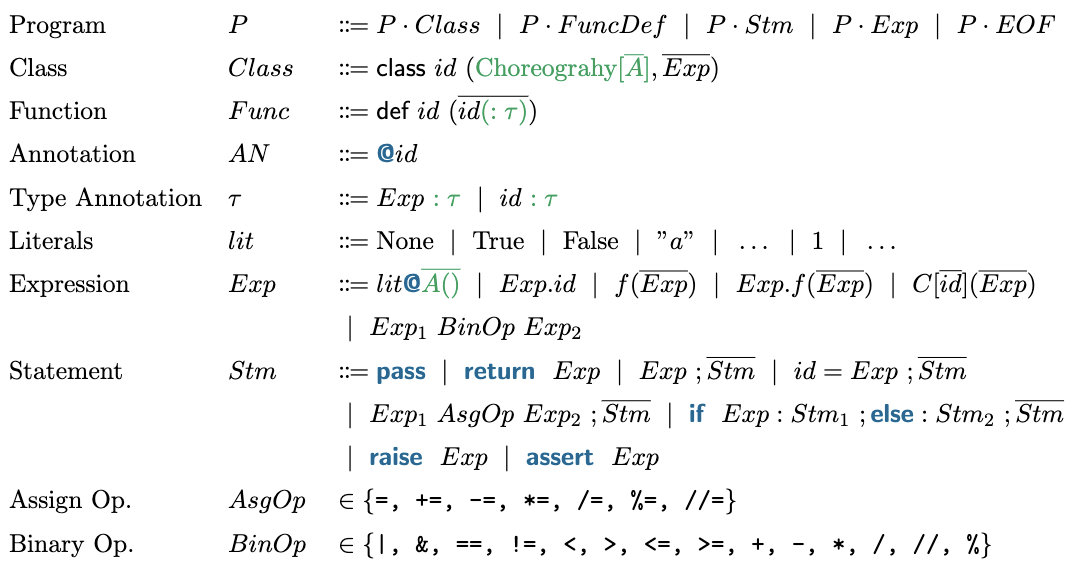
\includegraphics[scale=1.0]{image/syntax.png}
%  \caption{PyChoralの構文定義}
%\end{figure}

\subsection{merging}
\subsection{normalizing}

\section{実装}
\begin{itemize}
  \item typeshedの改造
  \item pro\_s, pro\_e, pro\_class, pro\_func
\end{itemize}
%%%%%%%%%%%%%%%%%%%%%%%%%%%%%%%%%%%%%%%%%%%%%%%%%%
%\chapter{評価}
%%%%%%%%%%%%%%%%%%%%%%%%%%%%%%%%%%%%%%%%%%%%%%%%%%
%\chapter{関連研究}
%%%%%%%%%%%%%%%%%%%%%%%%%%%%%%%%%%%%%%%%%%%%%%%%%%
\chapter{今後の課題}


%%%%%%%%%%%%%%%%%%%%%%%%%%%%%%
%\section*{謝辞}


%%%%%%%%%%%%%%%%%%%%%%%%%%%%%%%%%%%%%%%%%%%%%%%%%%
% 参考文献
%\begin{thebibliography}{99}
%\bibitem{OK13}
%  奥村 晴彦, 黒木 裕介,
%  [改訂第6版] LaTeX2$\epsilon$ 美文書作成入門,
%  技術評論社, 2013.
%\bibitem{Y02}
%  横尾 英俊,
%  LaTeXユーザのためのレポート・論文作成入門,
%  共立出版, 2002.
%\bibitem{Y08}
%  吉永 徹美,
%  独習 LaTeX2$\epsilon$
%  翔泳社, 2008.
%\end{thebibliography}
\chapter*{付録}
\section*{Projection to Python}

\begin{alignat*}{2}
  %%% ClassDef %%%
  &(Class)~~~ &&\projection{\textsf{class} ~id~(Ch(\overline{\cyan{B}}),\overline{Exp}):\overline{Stm}}{A}=
  \begin{cases}
    \textsf{class} ~id\_{\cyan{A}}~(\overline{\projection{Exp}{A}}):\overline{\projection{Stm}{A}} & \text{if}~~ {\cyan{A}} \in \overline{\cyan{B}}\\
    \text{absent} & \text{if}~~ {\cyan{A}} \notin \overline{\cyan{B}}
  \end{cases}\\
  \\
  %%% FuncDef %%%
  &(Func)~~~ &&\projection{\textsf{def} ~id~(\overline{id:TE}):\overline{Stm}}{A} = \textsf{def} ~id~ (\overline{id}):\overline{\projection{Stm}{A}}\\
  \\
  %%% Expression %%%
  &(Exp)~~~ &&\projection{lit\gray{@}(\overline{\color{cyan}{B}}):\tau}{A}=
  \begin{cases}
    lit & \text{if}~~ {\color{cyan}A} \in \overline{\color{cyan}{B}}\\
    \texttt{Unit.id} &\text{otherwise}
  \end{cases}\\
  %field
  &&&\projection{Exp.id:\tau}{A}=
  \begin{cases}
    \projection{Exp}{A}.id &\text{if}~~{\color{cyan}A} \in \text{rolesOf} (Exp.id)\\
    \text{absent} &\text{otherwise}
  \end{cases}\\
  %function
  &&&\projection{f(\overline{Exp}):\tau}{A} =
  \begin{cases}
    f(\overline{\projection{Exp}{A}}) &\text{if}~~ {\color{cyan}A} \in \text{rolesOf} (f(\overline{Exp}))\\
    \texttt{Unit.id}(f(\overline{\projection{Exp}{A}})) &\text{if}~~ {\color{cyan}A} \in \text{rolesOf}(\overline{Exp}) \wedge {\color{cyan}A} \notin \text{rolesOf} (f(\overline{Exp}))\\
    \texttt{Unit.id}(\overline{\projection{Exp}{A}}) &\text{otherwise}
  \end{cases}\\
  %method
  &&&\projection{Exp.f(\overline{Exp}):\tau}{A}=
  \begin{cases}
    \projection{Exp}{A}.f(\overline{\projection{Exp}{A}}) \\
    ~~~~~~~\text{if}~~ {\color{cyan}A} \in \text{rolesOf}(Exp) \wedge {\color{cyan}A} \in \text{rolesOf}(\overline{Exp})\\
    ~~~~~~~~~~~~~~~~~~~~~~~~~~~~~~~~ \wedge {\color{cyan}A} \in \text{rolesOf}(Exp.f(\overline{Exp}))\\
    \texttt{Unit.id}(\projection{Exp}{A}.f(\overline{\projection{Exp}{A}})) \\
    ~~~~~~~\text{if}~~ {\color{cyan}A} \in \text{rolesOf}(Exp) \wedge {\color{cyan}A} \notin \text{rolesOf}(Exp.f(\overline{Exp}))\\
    \texttt{Unit.id}(\projection{Exp}{A},\overline{\projection{Exp}{A}}) ~~~~~\text{otherwise}
  \end{cases}\\
  %create object
  &&&\projection{C[\overline{\color{cyan}B}](\overline{Exp}):\tau}{A}=
  \begin{cases}
    \projection{C[\overline{\color{cyan}B}]}{A} (\overline{\projection{Exp}{A}}) & {\color{cyan}A} \in \overline{\color{cyan}B}\\
    \texttt{Unit.id}(\overline{\projection{Exp}{A}}) &\text{otherwise}
  \end{cases}\\
  % binary operator
  &&&\projection{Exp_1 ~BinOp~ Exp_2}{A} = \projection{Exp_1}{A} ~BinOp~ \projection{Exp_2}{A}\\
  %role
  &&&\text{rolesOf}(\_:\tau\gray{@}(\overline{\color{cyan}B})) = {\overline{\color{cyan}B}}\\
  &&&\text{rolesOf}(\overline{Exp}) = \bigcup_i \text{rolesOf}(Exp_i) \\
  &&&\projection{\overline{Exp}}{A} = Exp'_1,Exp'_2,\cdots,Exp'_n ~~\text{where}~~ Exp'_i = \projection{Exp_i}{A}\\ 
  \\
  \\ 
  %%% Statement %%%
  %pass
  &(Stm)~~~ &&\projection{\gray{pass}}{A} = \gray{pass}\\
  %return
  &&&\projection{\gray{return} ~ Exp;}{A} = \gray{return} ~ \projection{Exp}{A}\\
  % e;s
  &&&\projection{Exp;\overline{Stm}}{A} =
  \begin{cases}
    \gray{match} ~\projection{Exp}{A}: \\
    ~~~~~\gray{case} ~id_2: \projection{\overline{Stm}}{A};~~~~~ \text{if}~~Exp = Exp'.\texttt{select}(id_1\gray{@}{\cyan{A}}.id_2):\texttt{Enum}\gray{@}{\cyan{A}}\\ %~~~ \text{Name}(f) = \texttt{Select}\\%&~~~~ {\cyan{A}} \in \text{rolesOf}(Exp.f(\overline{Exp})) ~~\text{and}\\
    ~~~~~\gray{case} ~\_\_: \text{assert False}; \\
    \projection{Exp}{A};\projection{\overline{Stm}}{A} ~~~~~ \text{otherwise}\\
  \end{cases}\\
  % Assignment 
  &&& \projection{id:TE = Exp~;\overline{Stm}}{A} =
  \begin{cases}
    id = \projection{Exp}{A};\projection{\overline{Stm}}{A} & \text{if}~~ {\color{cyan}A} \in \text{rolesOf}(TE)\\
    \projection{Exp}{A};\projection{\overline{Stm}}{A} & \text{otherwise}
  \end{cases}\\
  % OpAssignment
  &&& \projection{Exp_1 ~AsgOp~ Exp_2 ~; \overline{Stm}}{A} = \projection{Exp_1}{A} AsgOp~ \projection{Exp_2}{A} ~; \projection{\overline{Stm}}{A} \\
  % If
  &&&\projection{\gray{if}~Exp:Stm_1~;\gray{else}:Stm_2 ~;\overline{Stm}}{A}=\\
  &&&
  \begin{cases}
    \gray{if}~\projection{Exp}{A} : \projection{Stm_1}{A} ~; \gray{else}:\projection{Stm_2}{A} ~;\projection{\overline{Stm}}{A} & \text{if}~~ \text{rolesOf}(Exp) = \cyan{A}\\
    \projection{Exp}{A} ~; \nl{\projection{Stm_1}{A}} \mg \nl{\projection{Stm_2}{A}} ~;\projection{\overline{Stm}}{A} & \text{otherwise}
  \end{cases}\\
  % raise
  &&&\projection{\gray{raise}~Exp}{A} = \gray{raise}~\projection{Exp}{A}\\
  % assert
  &&&\projection{\gray{assert}~Exp}{A} = \gray{assert}~\projection{Exp}{A}\\
  % block
  &&&\projection{\overline{Stm}}{A} = Stm'_1,Stm'_2,\cdots,Stm'_n ~~\text{where}~~ Stm'_i = \projection{Stm_i}{A}\\  
\end{alignat*}

\section*{Merging}
\begin{align*}
  % Statement
  & \text{Statement}\\
  % stm_list
  & \overset{\color{red}.}{\mg} \overline{Stm} = \overset{\color{red}.}{\mg}(Stm_1, \cdots ,Stm_n) = \nl{Stm_1} \mg \cdots \mg \nl{Stm_n}\\
  % return
  & \gray{return}~Exp \mg \gray{return}~Exp' = \gray{return}~Exp \mg Exp'\\
  % raise
  & \gray{raise}~ Exp \mg \gray{raise}~ Exp' = \gray{raise}~ Exp \mg Exp'\\
  % assignment op
  & (Exp_1 ~AsgOp~ Exp_2 ; \overline{Stm}) \mg (Exp'_1 ~AsgOp~ Exp'_2 ; \overline{Stm'})\\
  & ~~~~~~~ = (Exp_1 \mg Exp'_1) ~AsgOp~ (Exp_2 \mg Exp'_2) ; (\overline{Stm} \mg \overline{Stm'})\\
  % expression stmt
  & (Exp ; \overline{Stm}) \mg (Exp' ; \overline{Stm'}) = (Exp \mg Exp') ; (\overline{Stm} \mg \overline{Stm'})\\
  % if 
  \\
  & \gray{if}~Exp_1: ~~~~~~~~~~~~~~~~~~~~\gray{if}~Exp'_1: ~~~~~~~~~~~~~~~~~~~~\gray{if}~Exp_1 \mg Exp'_1:\\
  & ~~~~~~Stm_1; ~~~~~~~~~~~~~~~~~~~~~~~~~ Stm'_1 ~~~~~~~~~~~~~~~~~~~~~~~~~~~ Stm_1 \mg Stm'_1\\
  & \cdots ~~~~~~~~~~~~~~~~~~~~~~~~~~~\cdots ~~~~~~~~~~~~~~~~~~~~~~~~~~~~\cdots\\
  & \gray{elif}~Exp_n: ~~~~~~\mg~~~~~~~\gray{elif}~Exp'_n: ~~~~~~~=~~~~~~~\gray{elif}~Exp_n \mg Exp'_n:\\
  & ~~~~~~Stm_n; ~~~~~~~~~~~~~~~~~~~~~~~~~~ Stm'_n ~~~~~~~~~~~~~~~~~~~~~~~~~~ Stm_n \mg Stm'_n\\
  & \gray{else}:~~~~~~~~~~~~~~~~~~~~~~~~\gray{else}:~~~~~~~~~~~~~~~~~~~~~~~~~\gray{else}:~\\
  & ~~~~~~Stm_e; ~~~~~~~~~~~~~~~~~~~~~~~~~~ Stm'_e ~~~~~~~~~~~~~~~~~~~~~~~~~~~ Stm_e \mg Stm'_e\\
  & \overline{Stm} ~~~~~~~~~~~~~~~~~~~~~~~~~~ \overline{Stm'} ~~~~~~~~~~~~~~~~~~~~~~~~~~ \overline{Stm} \mg \overline{Stm'}\\
  \\
  % match
  & \gray{match}~Exp: ~~~~~~~~~~~~~~~~~~~~\gray{match}~Exp': ~~~~~~~~~~~~~~~~~~~~\gray{match}~Exp \mg Exp':\\
  & ~~~\gray{case}~id_a : Stm'_a; ~~~~~~~~~~~~~~~~\gray{case}~id_a : Stm''_a; ~~~~~~~~~~~~~~~~\gray{case}~id_a : Stm'_a \mg Stm''_a;\\
  & ~~~\cdots ~~~~~~~~~~~~~~~~~~~~~~~~~~~~~~~~~\cdots ~~~~~~~~~~~~~~~~~~~~~~~~~~~~~~~~~~\cdots\\
  & ~~~\gray{case}~id_x : Stm'_x; ~~~~~~\mg~~~~~~\gray{case}~id_x : Stm''_x; ~~~~~~=~~~~~~\gray{case}~id_x : Stm'_x \mg Stm''_x;\\
  & ~~~\gray{case}~id_y : Stm'_y; ~~~~~~~~~~~~~~~~~~~~~~~~~~~~~~~~~~~~~~~~~~~~~~~~~~~~~~\gray{case}~id_y : Stm'_y; \\
  & ~~~~~~~~~~~~~~~~~~~~~~~~~~~~~~~~~~~~~~~~~\gray{case}~id_z : Stm'_z;~~~~~~~~~~~~~~~~\gray{case}~id_z : Stm'_z;\\
  & ~~~\gray{case}~~\_\_ ~: Stm'_{ex}; ~~~~~~~~~~~~~~~\gray{case}~~\_\_ ~: Stm''_{ex}; ~~~~~~~~~~~~~~~\gray{case}~~\_\_ ~:Stm'_{ex} \mg Stm''_{ex};\\
  & \overline{Stm} ~~~~~~~~~~~~~~~~~~~~~~~~~~~~~~~~~ \overline{Stm'} ~~~~~~~~~~~~~~~~~~~~~~~~~~~~~~~ \overline{Stm} \mg \overline{Stm'}\\
  \\
  & \overline{Stm} \mg \overline{Stm'} = Stm_1 \mg Stm_1'~,~Stm_2 \mg Stm_2'~,~\cdots~,Stm_n \mg Stm'_n\\
  \\
  % Expression
  & \text{Expression}\\
  & Exp \mg Exp' =
  \begin{cases}
    Exp & \text{if}~ Exp = Exp'\\
    \text{error} & \text{if}~ Exp \neq Exp'
  \end{cases}\\
\end{align*}

\section*{normalizer}
\begin{align*}
  % Statement
  & \text{Statements}\\
  & \nl{\gray{pass}} = \gray{pass}\\
  & \nl{\gray{return}~Exp} = \gray{return} ~ \nl{Exp}\\
  & {\scriptsize{\text{\color{Purple}NOOP}}}(Exp) = 
  \begin{cases}
    [blank] & \text{if}~~ Exp \in \{\texttt{Unit.id, None}\}\\
    Exp & \text{otherwise}
  \end{cases}\\
  & \nl{Exp_1 ~AsgOp~ Exp_2 ; \overline{Stm}} = 
  \begin{cases}
    \nl{Exp_1} ; \nl{\overline{Stm}} & \text{if}~~ {\scriptsize{\text{\color{Purple}NOOP}}}(\nl{Exp_2}) = [blank]\\
    \nl{Exp_2} ; \nl{\overline{Stm}} & \text{if}~~ {\scriptsize{\text{\color{Purple}NOOP}}}(\nl{Exp_1}) = [blank]\\
    \nl{\overline{Stm}} & \text{if}~~ {\scriptsize{\text{\color{Purple}NOOP}}}(\nl{Exp_1},\nl{Exp_2}) = [blank]\\
    \nl{Exp_1} AsgOp \nl{Exp_2} ; \nl{\overline{Stm}} & \text{otherwise}
  \end{cases}\\
  & \nl{Exp;\overline{Stm}} =
  \begin{cases}
    \nl{\overline{Stm}} & \text{if}~~ {\scriptsize{\text{\color{Purple}NOOP}}}(\nl{Exp}) = [blank]\\
    \nl{Exp} ; \nl{\overline{Stm}} & \text{otherwise}
  \end{cases}\\
  % Expression
  & \text{Expressions}\\
  & \nl{None} = None ~~~ \nl{id} = id 
\end{align*}

\end{document}